\documentclass{beamer}
\usepackage{hyperref}
\usepackage[CJKmath=true, AutoFakeBold = true]{xeCJK}
% \usepackage[T1]{fontenc}
\setCJKmainfont{AR PL KaitiM GB}
\usepackage{latexsym,xcolor,multicol,booktabs,calligra}
\usepackage{amssymb,amsfonts,amsmath,amsthm,mathrsfs,mathptmx}
\usepackage{graphicx,pstricks,listings,stackengine}
\usepackage[most]{tcolorbox}
\usefonttheme[onlymath]{serif}
\usepackage[brazil]{babel}

\renewcommand{\today}{19 de Junho de 2023}
\renewcommand{\alert}[1]{\textbf{\color{swufe}#1}}

\author[Rodrigues, J.]{Julio Cesar da Silva Rodrigues\inst{1}}
\title[Mineração de Dados - TP 2 - Final]{Identificando URLs maliciosas:}
\subtitle{Uma abordagem puramente léxica}
\institute[UFSJ]
{
    \inst{1} 
    Universidade Federal de São João del-Rei \\
    Curso de Ciência da Computação \\
    \textit{julio.csr.271@aluno.ufsj.edu.br}\\
    \vspace{0.35cm}
}

\date{27 de Junho de 2023}
\usepackage{SWUFE}

\def\cmd#1{\texttt{\color[RGB]{0, 0, 139}\footnotesize $\backslash$#1}}
\def\env#1{\texttt{\color[RGB]{0, 0, 139}\footnotesize #1}}

\lstset{
    language=[LaTeX]TeX,
    basicstyle=\ttfamily\footnotesize,
    keywordstyle=\bfseries\color[RGB]{0, 0, 139},
    stringstyle=\color[RGB]{50, 50, 50},
    numbers=left,
    numberstyle=\small\color{gray},
    rulesepcolor=\color{red!20!green!20!blue!20},
    frame=shadowbox,
}

\begin{document}

\begin{frame}
    \titlepage
    \vspace*{-1.5cm}
    \begin{figure}[htpb]
        \begin{center}
            
\includegraphics[width=0.4\linewidth]{pic/LogoUFSJ.PNG}
        \end{center}
    \end{figure}
\end{frame}

\begin{frame}
    \tableofcontents[sectionstyle=show,subsectionstyle=show/shaded/hide,subsubsectionstyle=show/shaded/hide]
\end{frame}

\section{Introdução}

\begin{frame}{Contextualização}

    \begin{itemize}
        \setlength{\itemsep}{10pt}
        \item Via rápida e direta para aplicar crimes cibernéticos;
        \item Potencial de infecção exponencial;
        \item Brasil no Top 15 com maior número de vítimas, segundo relatório\footnotemark \hspace{0.1cm}da Abranet;
        \item Evolução nas técnicas de camuflagem e detecção.
    \end{itemize}

    \footnotetext[1]{\tiny{Disponível em: \url{https://www.abranet.org.br/Noticias/Relatorio-aponta-que-cada-URL-maliciosa-no-Brasil-afeta-18-usuarios-2585.html?UserActiveTemplate=site}}}
    
\end{frame}

\begin{frame}{Objetivos}

    \begin{itemize}
        \setlength{\itemsep}{10pt}
        \item Principais características que definem a natureza de uma URL;
        \item Capacidade de predição analisando somente a estrutura léxica;
        \item Modelo competitivo com classificação multiclasse.
    \end{itemize}
    
\end{frame}

\section{Trabalhos Relacionados}

\begin{frame}{Classificação Multiclasse}
    
    \begin{itemize}
        \setlength{\itemsep}{10pt}
        \item Detecção de URLs baseada somente em atributos léxicos \cite{SALEEMRAJA2021163};
        \item Base de dados da UNB\footnotemark;
        \item Extração de 27 atributos;
        \item Cinco algoritmos de \emph{machine learning} selecionados;
        \item 99\% de acurácia com \emph{random forest}.
    \end{itemize}

    \footnotetext[2]{\tiny{University of New Brunswick}}
    
\end{frame}

\begin{frame}{Classificação Binária}

    \begin{itemize}
        \setlength{\itemsep}{10pt}
        \item Detecção de URLs de \emph{phishing} direcionadas a brasileiros \cite{sbrc};
        \item Aprendizado baseado em atributos léxicos e relacionados à rede;
        \item Bases de dados nacionais:
        \begin{enumerate}
            \vspace{0.2cm}
            \setlength{\itemsep}{10pt}
            \item CaUMa\footnotemark: URLs maliciosas;
            \item UFBA\footnotemark: URLs seguras.
        \end{enumerate}
    \end{itemize}

    \footnotetext[3]{\tiny{Serviço associado ao Catálogo de Fraudes da RNP}}
    \footnotetext[4]{\tiny{Universidade Federal da Bahia}}
    
\end{frame}

\begin{frame}{Classificação Binária}

    \begin{itemize}
        \setlength{\itemsep}{10pt}
        \item Extração de 117 características;
        \item Quatro algoritmos de \emph{machine learning} selecionados;
        \item Empate técnico com \emph{F1 Score} média de 95,85\%:
        \begin{enumerate}
            \vspace{0.2cm}
            \setlength{\itemsep}{10pt}
            \item KNN;
            \item SVM;
            \item J48. 
        \end{enumerate}
    \end{itemize}
    
\end{frame}

\section{Metodologia}

\begin{frame}{Base de Dados}
    
    \begin{itemize}
        \setlength{\itemsep}{10pt}
        \item Kaggle\footnotemark:
        \begin{enumerate}
            \vspace{0.2cm}
            \setlength{\itemsep}{10pt}
            \item Mais de 600 mil instâncias;
            \item 4 tipos de URL;
        \end{enumerate}
        \item PhishTank\footnotemark:
        \begin{enumerate}
            \vspace{0.2cm}
            \setlength{\itemsep}{10pt}
            \item Mais de 100 mil instâncias;
            \item Somente URLs de \emph{phishing};
        \end{enumerate}
    \end{itemize}

    \footnotetext[5]{\tiny Disponível em: \url{https://www.kaggle.com/datasets/sid321axn/malicious-urls-dataset}}
    \footnotetext[6]{\tiny Disponível em: \url{https://phishtank.org/phish_archive.php}}
    
\end{frame}

\begin{frame}{Base de Dados}
    
    \begin{figure}
        \centering
        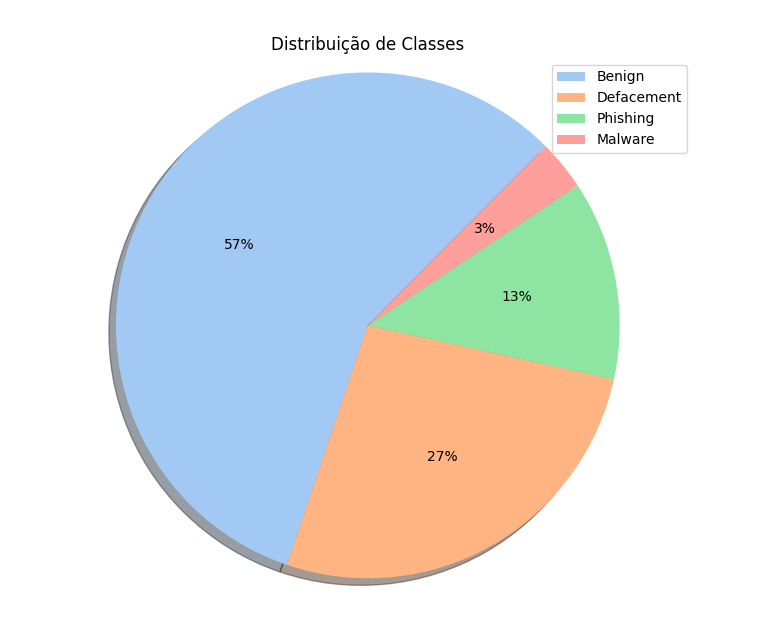
\includegraphics[width=0.85\textwidth]{pic/class.png}
        \label{fig:map1}
    \end{figure}
    
\end{frame}

\begin{frame}{Balanceamento}
    
    \begin{itemize}
        \setlength{\itemsep}{10pt}
        \item \emph{Undersampling} aleatório para instâncias \emph{benign};
        \item Redução de 428081 para 200 mil instâncias;
        \item \emph{Scraper} para coletar mais de 100 mil URLs da PhishTank;
        \item \emph{SMOTE} \cite{DBLP:journals/corr/abs-1106-1813} para suprir o déficit de instâncias de \emph{defacement} e \emph{malware}.
    \end{itemize}
    
\end{frame}

\begin{frame}{Construção de atributos}
    
    \begin{itemize}
        \setlength{\itemsep}{10pt}
        \item 21 atributos criados:
        \begin{enumerate}
            \vspace{0.2cm}
            \setlength{\itemsep}{10pt}
            \item 7 com base em análise estatística da base de dados;
            \item 14 criados utilizando trabalhos relacionados como base;
            \item Exemplos: \{Protocolo de comunicação, Comprimento da URL, Quantidade de \emph{tokens}, ...\}
        \end{enumerate}
        \item Aplicação de \emph{feature selection} com \textbf{RFECV};
    \end{itemize}
    
\end{frame}

\begin{frame}{Construção de atributos}
    
    \begin{figure}
        \centering
        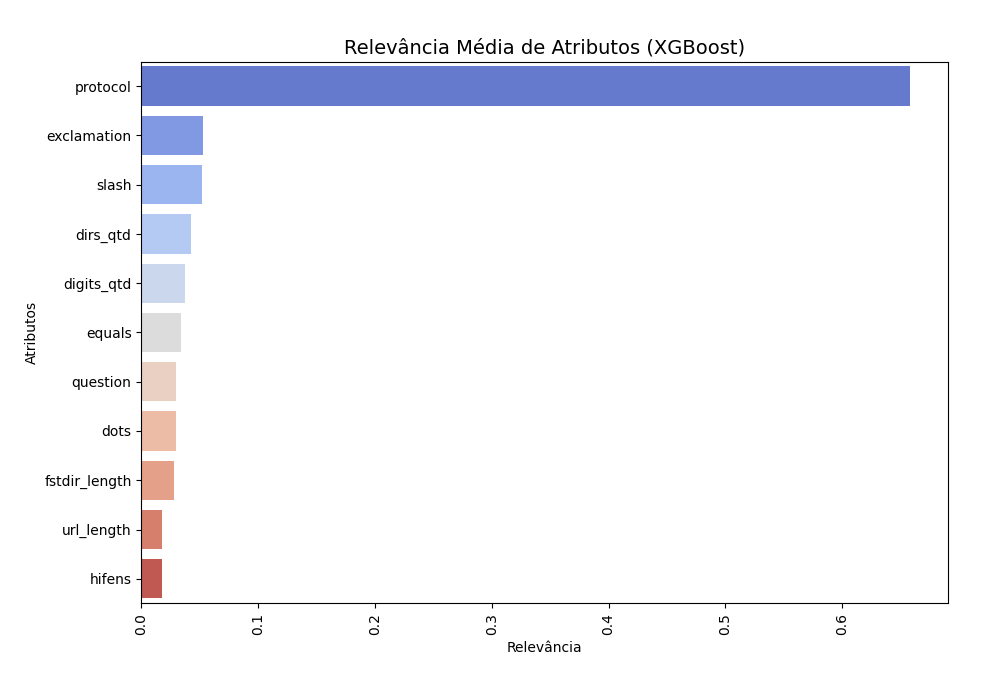
\includegraphics[width=1\textwidth]{pic/attr.png}
        \label{fig:map2}
    \end{figure}
    
\end{frame}

\begin{frame}{Base de Dados Final}
    
    \begin{itemize}
        \setlength{\itemsep}{10pt}
        \item 800 mil instâncias;
        \item Perfeitamente balanceada;
        \item 11 atributos e 1 classe (4 valores distintos);
        \item Composta por URLs de bases de dados do \emph{Kaggle} e \emph{PhishTank}.
    \end{itemize}
    
\end{frame}

\begin{frame}{Modelos de Aprendizado Supervisionado}
    
    \begin{itemize}
        \setlength{\itemsep}{10pt}
        \item Algoritmos selecionados:
        \begin{enumerate}
            \vspace{0.2cm}
            \setlength{\itemsep}{10pt}
            \item XGBoost;
            \item KNN;
            \item Regressão Logística.
        \end{enumerate}
        \item Validação cruzada com amostragem estratificada (\emph{10-fold});
        \item Métrica \emph{Macro F1} e desvio padrão;
        \item Ajuste fino - \emph{Tripartite} (\emph{5-fold});
        \item Teste t de dupla cauda.
    \end{itemize}
    
\end{frame}

\section{Resultados}

\begin{frame}{Comparativo de Algoritmos}
    
\begin{table}
\centering
\caption{\emph{Macro F1 Scores} alcançadas pelos algoritmos}
\vspace*{-0.5cm}
\resizebox{\columnwidth}{!}{
\begin{tabular}{|c|c|c|}

%\begin{tabularx}{\columnwidth}{|lcccc|}
\hline 
 
\multicolumn{3}{|c|}{Resultados}\\ 
\hline

 Algoritmo & Média  & Desvio Padrão\\
 \hline 
 %\rowcolor{Gray}
%\multicolumn{5}{|c|}{Dictionary} \\ 
% \hline 
Regressão Logística & 0,7339 & 0,0039\\   %\hdashline
XGBoost & 0,9476 & 0,0006\\  %\hdashline  
KNN & 0,9229 & 0,0008\\
  \hline 


\end{tabular}
}
%\end{tabularx}
%\label{se:Dic}
\end{table}

    \begin{itemize}
        \setlength{\itemsep}{10pt}
        \item XGBoost e KNN com desempenho similar inicialmente;
        \item Desvio padrão constantemente baixo é um bom indicativo.
    \end{itemize}
    
\end{frame}

\begin{frame}{Teste Estatístico}

    \begin{itemize}
        \setlength{\itemsep}{10pt}
        \item Nível de significância \(\rightarrow \alpha = 0,05\);
        \item XGBoost x KNN:
        \begin{enumerate}
            \vspace{0.2cm}
            \setlength{\itemsep}{10pt}
            \item Hipótese nula rejeitada;
            \item Modelos estatisticamente distintos.
        \end{enumerate}
        \item XGBoost x Regressão Logística:
        \begin{enumerate}
            \vspace{0.2cm}
            \setlength{\itemsep}{10pt}
            \item Hipótese nula rejeitada;
            \item Modelos estatisticamente distintos.
        \end{enumerate}
    \end{itemize}
    
\end{frame}

\begin{frame}{Teste Estatístico}

    \begin{itemize}
        \setlength{\itemsep}{10pt}
        \item KNN x Regressão Logística:
        \begin{enumerate}
            \vspace{0.2cm}
            \setlength{\itemsep}{10pt}
            \item Hipótese nula rejeitada;
            \item Modelos estatisticamente distintos.
        \end{enumerate}
        \item XGBoost na dianteira como o melhor desempenho;
        \item Alta disparidade em custo computacional.
    \end{itemize}
    
\end{frame}

\begin{frame}{Limitações}

    \begin{figure}
        \centering
        \vspace*{-0.3cm}
        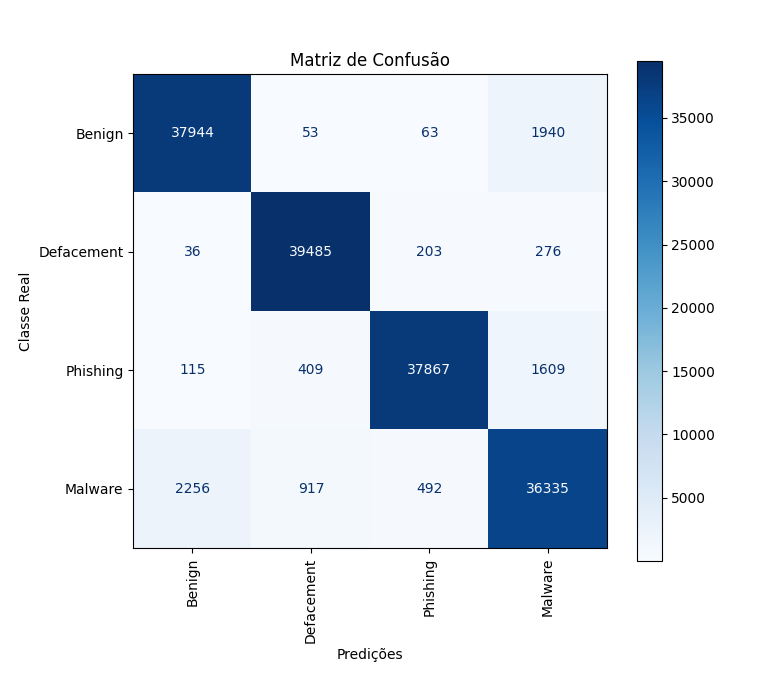
\includegraphics[width=0.8\textwidth]{pic/confusion.png}
        \label{fig:map4}
    \end{figure}
    
\end{frame}


\begin{frame}{Limitações}

    \begin{figure}
        \centering
        \vspace*{-0.3cm}
        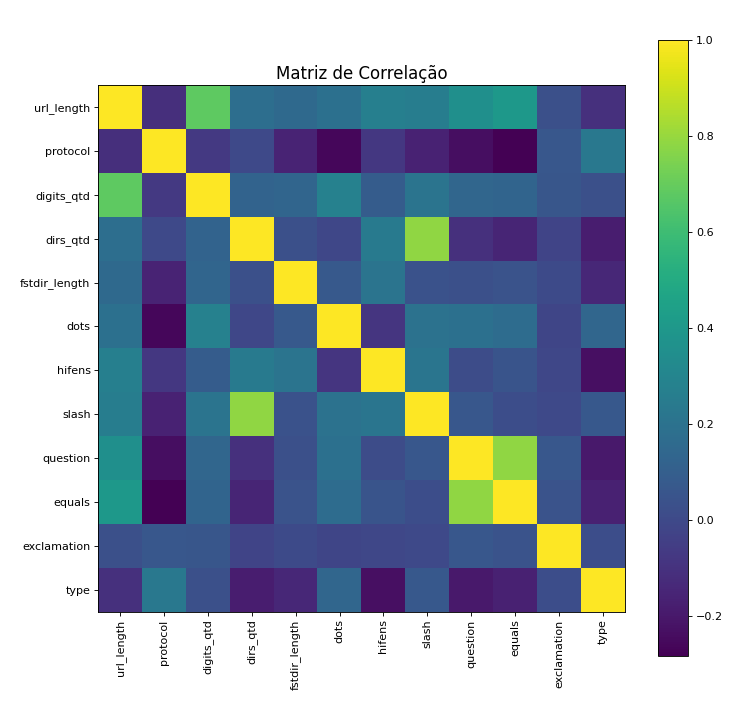
\includegraphics[width=0.78\textwidth]{pic/corr.png}
        \label{fig:map4}
    \end{figure}
    
\end{frame}

\section{Conclusão}

\begin{frame}{Considerações Finais}

    \begin{itemize}
        \setlength{\itemsep}{10pt}
        \item Distinção entre URLs maliciosas;
        \item Potencial para competir com modelos que utilizam outros tipos de características;
        \item Generalização e nível de confiabilidade na classificação.
    \end{itemize}
    
\end{frame}

\begin{frame}{Passos Futuros}

    \begin{itemize}
        \setlength{\itemsep}{10pt}
        \item Exploração mais profunda na construção de atributos;
        \item Investigação minunciosa sobre o que separa \emph{malware} de outros tipos de URL;
        \item Possíveis reduções no volume da base de dados (\emph{instance selection?}).
    \end{itemize}
    
\end{frame}

\section*{Final}

\begin{frame}{Referências}
    \scriptsize\bibliographystyle{apalike}
    \bibliography{ref}
\end{frame}

\end{document}